%%% ======= Beamer ======
\documentclass[usenames,dvipsnames,t]{beamer}
% \documentclass[usenames,dvipsnames, handout]{beamer}
\beamertemplatenavigationsymbolsempty % remove toolbar at the bottom of slides
\usepackage{appendixnumberbeamer} % for appendix
\usetheme{Madrid}
\usecolortheme{default}
\useinnertheme{circles}

\usepackage{fontawesome}

% Define commands for social media icons with links
\newcommand{\twitter}{\href{https://twitter.com/ThibeauWouters}{\textcolor{black}{\faTwitter}}}
\newcommand{\linkedin}{\href{https://www.linkedin.com/in/ThibeauWouters}{\textcolor{black}{\faLinkedin}}}
\newcommand{\github}{\href{https://github.com/ThibeauWouters}{\textcolor{black}{\faGithub}}}

\setbeamercolor{author in head/foot}{bg=blue!10, fg=blue}
\setbeamercolor{title in head/foot}{bg=blue!10, fg=blue}
\setbeamercolor{date in head/foot}{bg=blue!10, fg=blue}

\makeatletter
\setbeamertemplate{footline}{
  \leavevmode%
  \hbox{%
  \begin{beamercolorbox}[wd=.333333\paperwidth,ht=2.25ex,dp=1ex,center]{author in head/foot}%
    \usebeamerfont{author in head/foot}\insertshortauthor\expandafter\ifblank\expandafter{\beamer@shortinstitute}{}{~~(\insertshortinstitute)}
  \end{beamercolorbox}%
  \begin{beamercolorbox}[wd=.333333\paperwidth,ht=2.25ex,dp=1ex,center]{title in head/foot}%
    \usebeamerfont{title in head/foot}\insertshorttitle
  \end{beamercolorbox}%
  \begin{beamercolorbox}[wd=.333333\paperwidth,ht=2.25ex,dp=1ex,right]{date in head/foot}%
    \usebeamerfont{date in head/foot}\insertshortdate{}\hspace*{2em}
    \insertframenumber{}%
%     / \inserttotalframenumber
    \hspace*{2ex} 
  \end{beamercolorbox}}%
  \vskip0pt%
}
\makeatother

\colorlet{beamer@blendedblue}{blue!70} % change color theme

\usepackage[style=numeric-comp,sorting=none,backend=biber]{biblatex}%<- specify style
\addbibresource{references.bib}%<- specify bib file

\usepackage{svg}


% For appendix
\newcommand{\backupbegin}{
   \newcounter{framenumberappendix}
   \setcounter{framenumberappendix}{\value{framenumber}}
}
\newcommand{\backupend}{
   \addtocounter{framenumberappendix}{-\value{framenumber}}
   \addtocounter{framenumber}{\value{framenumberappendix}} 
}

\setbeamertemplate{bibliography item}{\insertbiblabel} % improved references



% Other preamble stuff:
\usepackage{preamble}

%%% Uncomment for another color palette
% \definecolor{Logo1}{rgb}{0.0, 0, 0.7}
% \definecolor{Logo2}{rgb}{2.55, 2.55, 2.55}

% \setbeamercolor*{palette primary}{bg=Logo1, fg=white}
% \setbeamercolor*{palette secondary}{bg=Logo2, fg=white}
% \setbeamercolor*{palette tertiary}{bg=white, fg=Logo1}
% \setbeamercolor*{palette quaternary}{bg=white,fg=white}
% \setbeamercolor{structure}{fg=Logo1} % itemize, enumerate, etc
% \setbeamercolor{section in toc}{fg=Logo1} % TOC sections

% For figures
\usepackage{import}
\usepackage{xifthen}
\usepackage{pdfpages}
\usepackage{transparent}
\usepackage{mdframed}
\usepackage{subcaption}

\setbeamertemplate{caption}[numbered]



% --- Inkscape figures:
\newcommand{\incfig}[2][0.75\textwidth]{%
    \def\svgwidth{\columnwidth}
    \resizebox{#1}{!}{\import{Inkscape figs/}{#2.pdf_tex}}
}

% --- Height of frame
\newlength{\myheight}
\setlength{\myheight}{7cm}

\newlength\myheightfigureintext
\newlength\mydepthfigureintext
\settototalheight\myheightfigureintext{Xygp}
\settodepth\mydepthfigureintext{Xygp}
\setlength\fboxsep{0pt}


%------------------------------------------------------------
%This block of code defines the information to appear in the
%Title page
\title[XMXS] %optional %  [arXiv:2404.11397]
{Accelerated Bayesian inference of multimessenger astronomy with \texttt{jax} and machine learning}

\author[Thibeau Wouters]{\small{\textbf{Thibeau Wouters}, Peter T. H. Pang, Chris Van Den Broeck} \\ \vspace{2mm} \href{mailto:t.r.i.wouters@uu.nl}{t.r.i.wouters@uu.nl} \newline \github \quad \linkedin \quad \twitter} % \\ \vspace{7mm} \href{http://arxiv.org/abs/2404.11397}{arXiv:2404.11397}

% \raisebox{-\mydepthfigureintext}{\fbox{
\includegraphics[height=\myheightfigureintext]{Figures/arxiv_logo_red_no_background.png}}}

\date{23 -- 27 September 2024}




%End of title page configuration block
%------------------------------------------------------------



%------------------------------------------------------------
%The next block of commands puts the table of contents at the 
%beginning of each section and highlights the current section:

\AtBeginSection[]
{
  \begin{frame}[plain, noframenumbering]
    \frametitle{Table of Contents}
    \tableofcontents[currentsection]
  \end{frame}
}


%------------------------------------------------------------


\begin{document}

{

  \usebackgroundtemplate{\transparent{0.15}{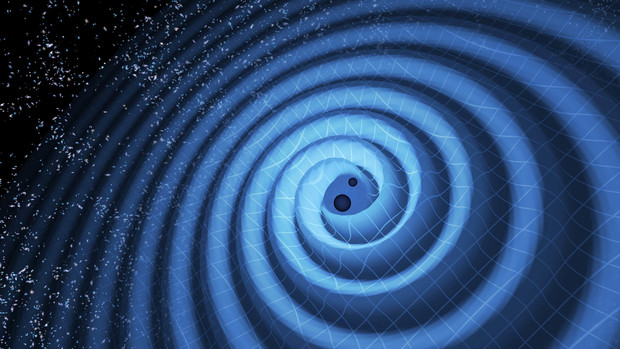
\includegraphics[width=\paperwidth,height=\paperheight]{Figures/GW-2.jpeg}}}
  % \usebackgroundtemplate{\transparent{0.15}{\includegraphics[width=\paperwidth,height=\paperheight]{Figures/XMXS_po}}}
  
\begin{frame}[plain, noframenumbering]
\titlepage

\begin{columns}
  \column{0.35\textwidth}
  \begin{figure}
    \centering
    \vspace{1.5mm}
    
\includegraphics[width=0.75\linewidth]{Figures/utrecht-university.png}
  \end{figure}
  \column{0.35\textwidth}
  \begin{figure}
    \centering
    
\includegraphics[width=0.75\linewidth]{Figures/Nikhef_logo-transparent.png}
  \end{figure}
\end{columns}

\end{frame}
}

% %The next statement creates the title page.
% \frame[plain]{\titlepage

%---------------------------------------------------------
%This block of code is for the table of contents after
%the title page
% \begin{frame}[plain, noframenumbering]
% \frametitle{Table of Contents}
% \tableofcontents
% \end{frame}
%---------------------------------------------------------


% \section{Gravitational waves from binary neutron star}

\begin{frame}{\texttt{N}uclear \texttt{M}ulti-\texttt{M}essenger \texttt{A}strophysics}

  \def\x{7mm}
  \def\y{3mm}
  
  \begin{itemize}
    \item \texttt{NMMA}: \texttt{N}uclear \texttt{M}ulti-\texttt{M}essenger \texttt{A}strophysics (Peter T.H. Pang) 
    % \vspace{\y}
    % \begin{itemize}
    %   \item \url{https://github.com/nuclear-multimessenger-astronomy/nmma}
    % \end{itemize}
    
    \vspace{\x}

    \item A Pythonic library for probing nuclear physics and cosmology with multimessenger analysis
    % \begin{itemize}
    %   \item Gravitational waves, kilonovae, gamma-ray bursts
    % \end{itemize}
    
    \vspace{\x}

    \item Used for overview of EOS constraints, with ``precomputed'' EOS set (\href{https://arxiv.org/abs/2402.04172}{arXiv:2402.04172})
    \begin{itemize}
      \item Metamodel
      \item Speed-of-sound extension scheme
    \end{itemize}
  \end{itemize}

  \vspace{\x}

  \begin{tcolorbox}[colback=blue!10, boxrule=0pt]
    \textbf{Next step:} Infer EOS parameters directly from multimessenger data
  \end{tcolorbox}
  
  \end{frame}


% \begin{frame}{Gravitational waves from binary neutron stars}

%   \def\x{5mm}
  
%   The EOS predicts the relation between mass $M$ and radius $R$ or \red{tidal deformability} of neutron stars.

%   \vspace{\x}

%   We can infer the tidal deformability of neutron stars from \red{gravitational wave signals} emitted by binary neutron star mergers.

%   \vspace{\x}
  
%   \begin{figure}
%     \centering
%     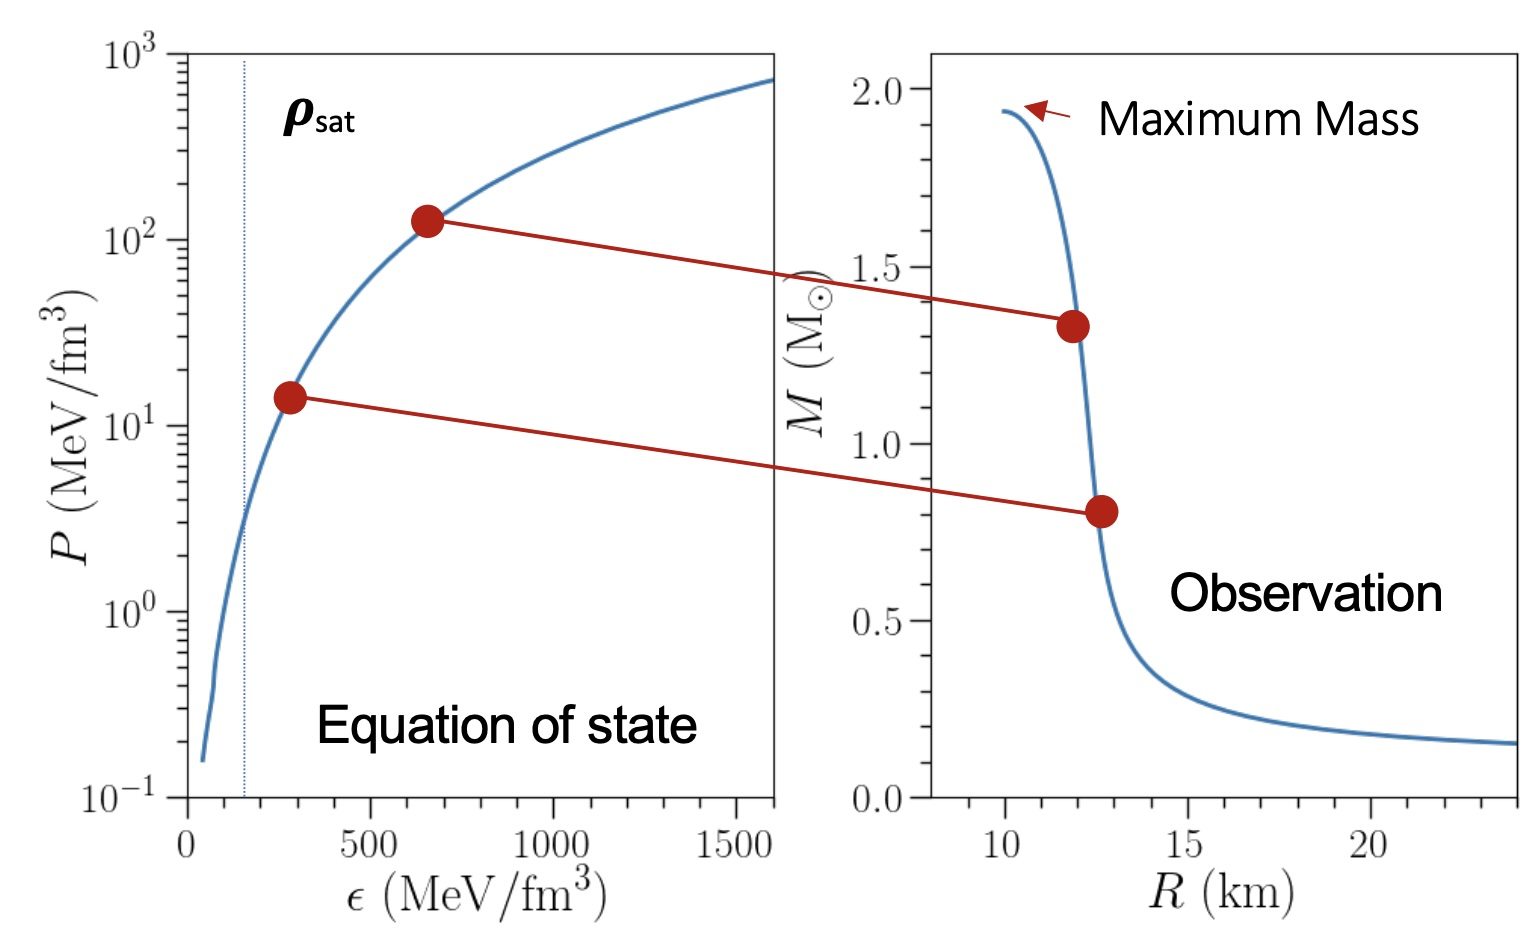
\includegraphics[width=0.60\textwidth]{Figures/ingo_eos_TOV_without_TOV.jpg}
%     \caption*{}
%   \end{figure}
  
%   \end{frame}

\begin{frame}{Bayesian inference}

\def\x{4mm}
\def\y{2mm}

Bayesian inference: get \textcolor{ForestGreen}{posterior} of parameters $\theta$ from data $d$ % ($13$ to $17$ parameters) from gravitational wave data $d$:
\begin{equation*}
    \textcolor{ForestGreen}{p(\theta | d)} = \frac{p(d | \theta) p(\theta)}{p(d)} = \frac{\text{likelihood} \times \text{prior}}{\text{evidence}}
\end{equation*}

\vspace{\x}

\begin{tcolorbox}[colback=blue!10, boxrule=0pt]
  \textbf{Problem:} Prohibitively expensive with multimessenger data 
\end{tcolorbox}

\begin{figure}
  \centering
  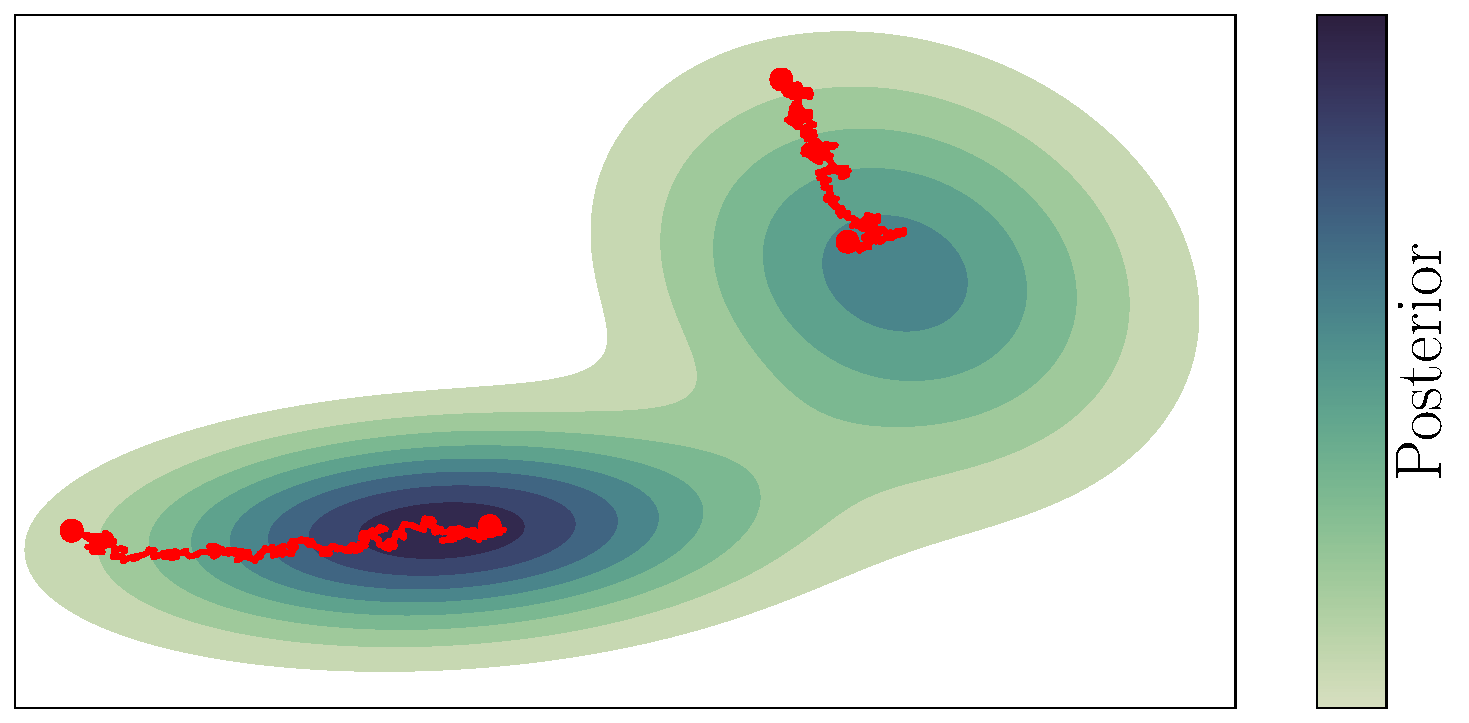
\includegraphics[width=0.60\textwidth]{Figures/mixture_of_gaussians_projection_no_title_colorbar.pdf}
  \caption*{}
\end{figure}

\end{frame}

\begin{frame}{\textsc{jax} and normalizing flows}

  \def\x{4mm}
  \def\y{2mm}
  \def\z{0.75cm}
  
  % \begin{tcolorbox}[colback=blue!10, boxrule=0pt]
  %   What are the benefits of \textsc{jax} for MCMC?
  % \end{tcolorbox}
  
  
  \textsc{jax} = \textsc{Numpy} $+$ composable transformations: 
  \begin{columns}
    \column{0.75\textwidth}
    \begin{enumerate}
      \item Automatic differentiation
      
      \vspace{\x}
      
      \item Just-in-time (JIT) compilation
      
      \vspace{\x}
      
      \item GPU acceleration
      
      \vspace{\x}
      
      \item Parallelization
  \end{enumerate}
  \column{0.20\textwidth}
  \begin{figure}
    % \centering
    
\includegraphics[width=\textwidth]{Figures/jax.png}
  \end{figure}
\end{columns}

\vspace{\z}
\hrule 
\vspace{\z}

% \vspace{\z}

\textbf{Normalizing flows}: generative deep learning model to approximate target distribution

\end{frame}  


\begin{frame}{Accelerating Bayesian inference for MMA: progress}

  \def\x{4mm}
  \def\y{2mm}

  \begin{itemize}

    \item Gravitational waves: 
    \vspace{\y}
    \begin{itemize}
      \item Analyze binary neutron stars in \red{15 -- 30 minutes} rather than $\mathcal{O}(\rm{hours})$ (\href{https://arxiv.org/abs/2404.11397}{arXiv:2404.11397})
      
      \vspace{\y}
      
      \item \faGithub~\href{https://github.com/kazewong/jim}{\texttt{kazewong/jim}}
    \end{itemize}

    \vspace{\x}
    
    % \item \texttt{Jim}: Accelerate Bayesian inference with (i) \texttt{jax} and (ii) normalizing flows (machine learning) (arXiv:2404.11397)
    % \begin{itemize}
    %   \item \url{https://github.com/kazewong/jim/}
      
    %   \item Sampler: \texttt{flowMC} (\url{https://github.com/kazewong/flowMC})
    % \end{itemize}
    
    % \vspace{\x}

    % \item Result: \red{$\sim 30$ minutes} on a single GPU
    
    % \vspace{\x}

    % \item Enable large-scale simulations on EOS constraints from gravitational waves

    \item TOV solver: 
    \vspace{\y}
    \begin{itemize}
      \item \red{10 -- 100 $\times$} faster
      
      \vspace{\y}
      
      \item \faGithub~\href{https://github.com/tsunhopang/jose}{\texttt{tsunhopang/jose}}
    \end{itemize}

    \vspace{\x}

    \item Kilonovae, GRBs: \faGithub~\href{https://github.com/ThibeauWouters/fiesta}{\texttt{ThibeauWouters/fiesta}}

    \vspace{\x}

    \item Ongoing: 
    \vspace{\y}
    \begin{itemize}
      \item Next-generation gravitational wave detectors
      
      \vspace{\y}

      \item Combine into one multimessenger analysis pipeline
    \end{itemize}
  \end{itemize}


\end{frame}


\end{document}

